\documentclass[aspectratio=169]{beamer}

\usepackage[utf8]{inputenc}
\usepackage{lmodern}
\usepackage{booktabs}
\usepackage{xcolor}
\usepackage{hyperref}
\usepackage{graphicx}

\usetheme{metropolis}
\metroset{block=fill, progressbar=frametitle}

\definecolor{ok}{HTML}{2ecc71}
\definecolor{alert}{HTML}{e74c3c}
\definecolor{subtle}{HTML}{7f8c8d}

\title{Missense Variant Pathogenicity Classification}
\subtitle{An Honest Baseline with Paralog-Aware Evaluation}
\author{Rayan AlShahrani}
\institute{King Khalid University \\ Computer Science Graduation Project}
\date{2026}

\begin{document}

% ═════════════════════════════════════════════════════════════════════════
\maketitle

% Slide 2 — The one-sentence pitch
\begin{frame}{The pitch, in one sentence}
  \vspace{0.6cm}
  \centering
  \large We built a missense-variant classifier that reports the
  \\ \vspace{0.3em} \emph{honest} number, not the \emph{inflated}
  one --- \\[0.6em]
  \large and showed exactly where the pre-audit baseline lied,
  \\ measured by how much.
\end{frame}

% ═════════════════════════════════════════════════════════════════════════
% Part 1: The problem
% ═════════════════════════════════════════════════════════════════════════

\section{The problem}

\begin{frame}{What is a missense variant?}
  \begin{itemize}
    \item Single nucleotide change $\to$ different amino acid in one
          protein.
    \item Ranges from silent to catastrophic.
    \item $\sim$90\% of observed missense variants have \emph{unknown}
          clinical significance.
    \item Clinical genomics needs a tool that says: \\
          \alert{``this variant is likely pathogenic, at this confidence
          level''}.
  \end{itemize}
\end{frame}

\begin{frame}{Why is it hard?}
  \begin{itemize}
    \item Only $\sim$2\% of observed missense variants have
          high-confidence ClinVar classifications.
    \item The true functional status has never been assayed for
          the remaining $\sim$98\%.
    \item Supervised models rely on \emph{circumstantial evidence}
          --- conservation, chemistry, population frequency.
    \item Three failure modes in prior work:
    \begin{enumerate}
      \item Definitional circularity (``common $\Rightarrow$ benign''
            as a feature).
      \item Meta-predictor contamination (using REVEL/CADD as
            features when they're trained on ClinVar).
      \item \alert{Paralog leakage} (KRT1 in train, KRT14 in test
            $\to$ 80\% sequence identity).
    \end{enumerate}
  \end{itemize}
\end{frame}

% ═════════════════════════════════════════════════════════════════════════
% Part 2: The audit
% ═════════════════════════════════════════════════════════════════════════

\section{The audit}

\begin{frame}{We audited our own baseline}
  \begin{block}{Pre-audit numbers}
    \centering
    \large ROC-AUC \textbf{0.955} \qquad PR-AUC \textbf{0.955}
  \end{block}

  \vspace{0.6em}
  \begin{itemize}
    \item Too flat across splits.
    \item Too high relative to published benchmarks.
    \item \alert{Suspicious ceiling} $\to$ investigate.
  \end{itemize}
\end{frame}

\begin{frame}{Leakage source 1: non-missense rows}
  \centering
  \large 64\% of pathogenic rows had null \texttt{ref\_aa} or
  \texttt{alt\_aa}.

  \vspace{1em}
  \begin{itemize}
    \item Stop-gained, splice-site, UTR variants leaking into a
          ``missense'' dataset.
    \item Model learned the shortcut:
          \emph{null AA features $\Rightarrow$ pathogenic}.
    \item Fix: \texttt{ref\_aa AND alt\_aa NOT NULL} filter.
  \end{itemize}
  \vspace{1em}
  \begin{alertblock}{Impact}
    PR-AUC \textbf{0.955} $\to$ \textbf{0.819}
    (the biggest single drop)
  \end{alertblock}
\end{frame}

\begin{frame}{Leakage source 2: feature hygiene}
  \begin{itemize}
    \item \texttt{is\_common} $=$ ``AF\_popmax $>$ 0.01''.
          \\ By ClinVar convention: \alert{100\% benign} when True.
          \\ $\Rightarrow$ definitional circularity.
    \item \texttt{chr} one-hot: 15\% gain came from
          dataset-composition artifact (chr17 over-represents BRCA1
          pathogenic variants, etc.), not biology.
    \item Both removed. Enforced by CI gate on every push.
  \end{itemize}
  \vspace{0.4em}
  \begin{alertblock}{Impact}
    PR-AUC \textbf{0.819} $\to$ \textbf{0.816}
    (small in magnitude, large in interpretive value)
  \end{alertblock}
\end{frame}

\begin{frame}{Leakage source 3: paralog leakage}
  \begin{itemize}
    \item Plain gene-level split seems safe.
          But 52\% of gene-prefix families (ZNF*, SLC*, KRT*, TMEM*)
          were shared between train and test.
    \item Keratin paralogs share $>$80\% sequence identity.
          KRT1 in train $\Rightarrow$ model effectively saw KRT14.
    \item Fix: \alert{family-level} split.
          16 curated regex patterns + trailing-digit fallback.
          15{,}479 genes $\to$ 7{,}851 families.
    \item Zero shared families across splits (CI-enforced).
  \end{itemize}
\end{frame}

\begin{frame}{The five-stage journey}
  \centering
  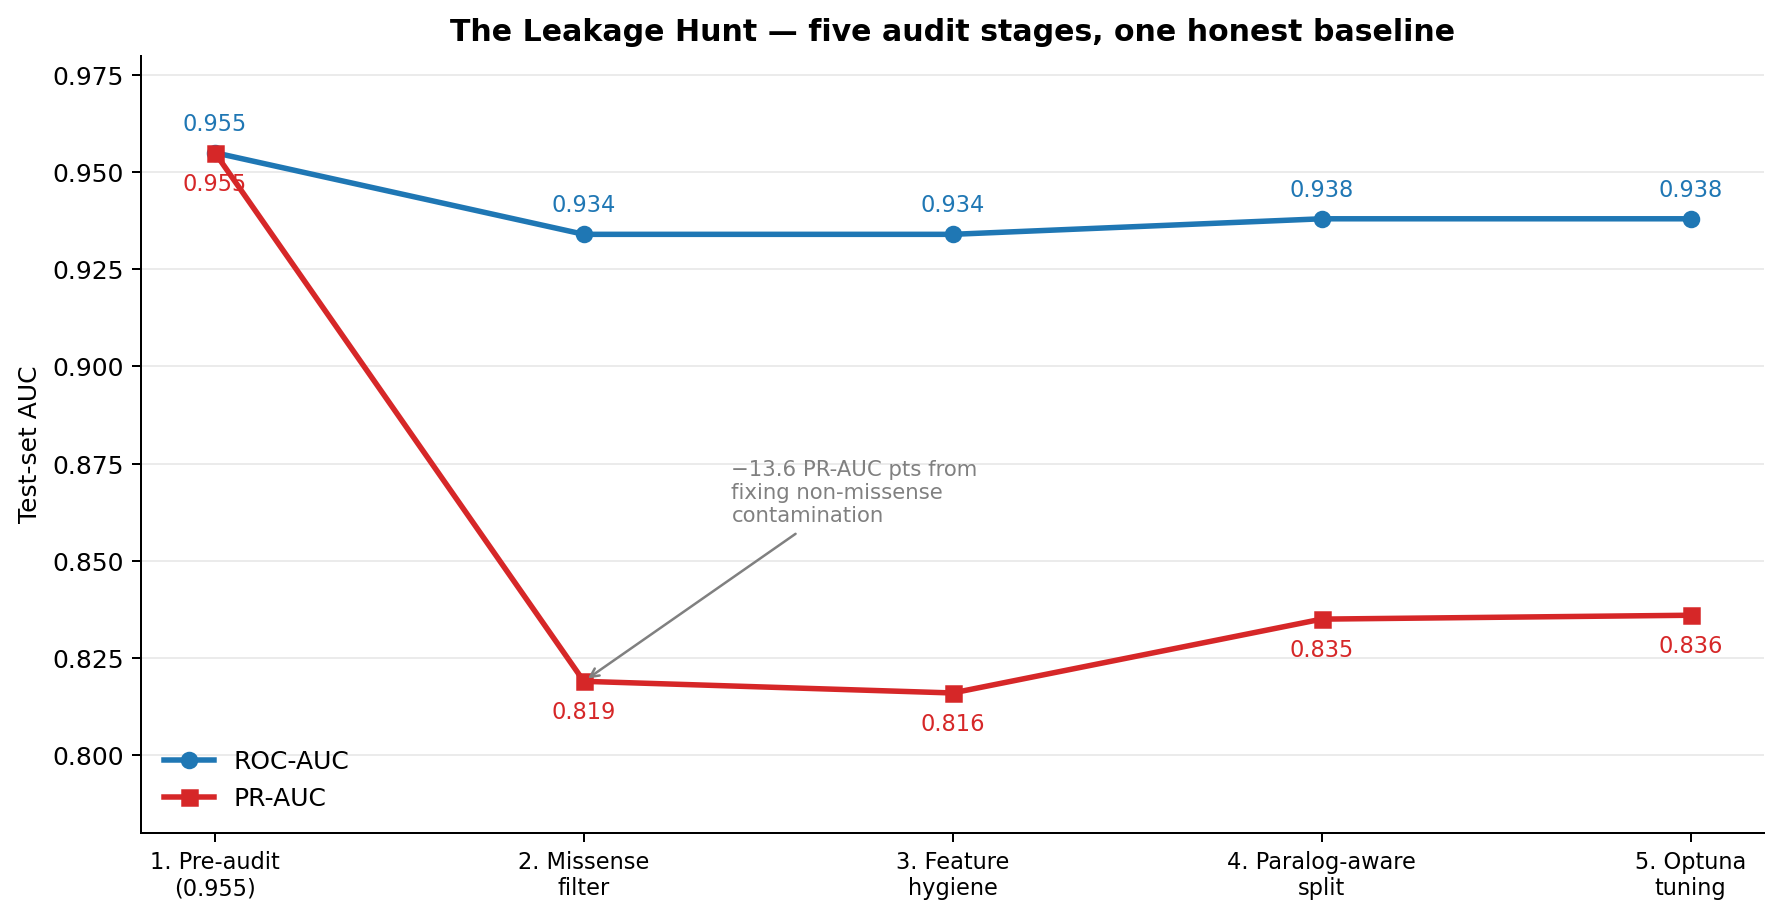
\includegraphics[width=\linewidth]{figures/leakage_journey.png}
\end{frame}

\begin{frame}{Post-audit}
  \begin{block}{Honest numbers (ClinVar test, paralog-disjoint)}
    \centering
    \large ROC-AUC \textbf{0.938} [0.935, 0.941] \\
    \large PR-AUC \textbf{0.838} [0.830, 0.846] \\
    \large ECE (calibrated) \textbf{0.011}
  \end{block}
  \vspace{0.5em}
  \begin{itemize}
    \item All 95\% CIs from 1{,}000-replicate bootstrap.
    \item No banned features in the training matrix (CI-enforced).
    \item 158 pytest tests green on every push.
  \end{itemize}
\end{frame}

% ═════════════════════════════════════════════════════════════════════════
% Part 3: Baseline comparison
% ═════════════════════════════════════════════════════════════════════════

\section{Baseline comparison}

\begin{frame}{Published tools on \textbf{our} test split}
  Every baseline scored on the same paralog-disjoint test.
  1{,}000-bootstrap 95\% CIs.
  \vspace{0.5em}

  \small
  \centering
  \begin{tabular}{@{} l r l l r @{}}
    \toprule
    Method & Year & ROC-AUC & PR-AUC & Cov. \\
    \midrule
    SIFT              & 2003 & 0.881 [0.877, 0.885] & 0.620 [0.610, 0.629] & 96\% \\
    PolyPhen-2        & 2010 & 0.893 [0.888, 0.898] & 0.728 [0.716, 0.739] & 93\% \\
    \textbf{XGBoost (ours)} & 2026 & \textbf{0.938} & \textbf{0.838} & \textbf{100\%} \\
    AlphaMissense$^*$ & 2023 & 0.956 [0.953, 0.958] & 0.890 [0.882, 0.898] & 86\% \\
    \bottomrule
  \end{tabular}
  \vspace{0.5em}
  \\
  \footnotesize $^*$ calibrated on ClinVar at release $\Rightarrow$
  inflated here.
\end{frame}

\begin{frame}{Baseline forest plot}
  \centering
  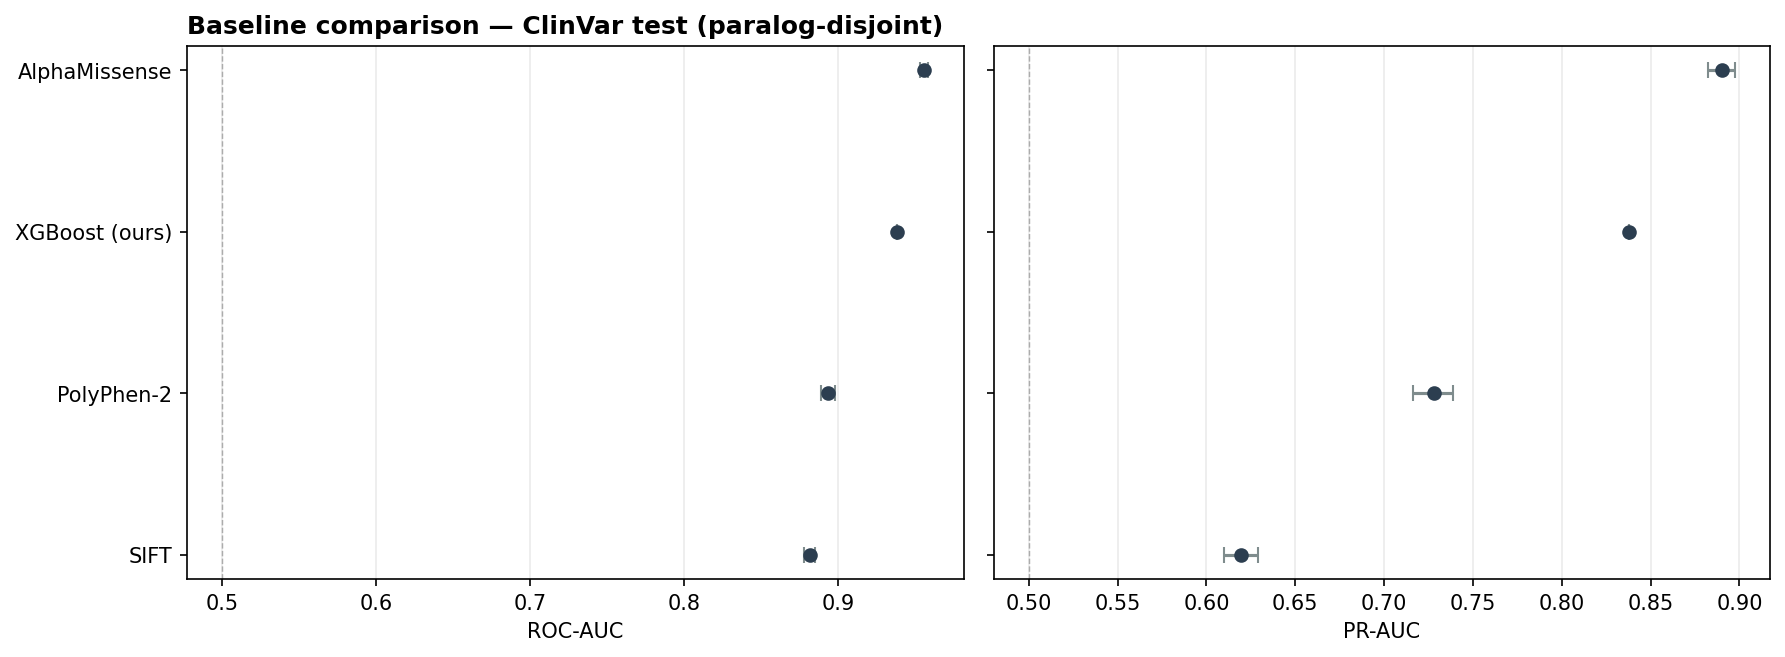
\includegraphics[width=0.93\linewidth]{figures/baselines_forest_plot.png}
\end{frame}

% ═════════════════════════════════════════════════════════════════════════
% Part 4: Calibration
% ═════════════════════════════════════════════════════════════════════════

\section{Calibration}

\begin{frame}{Why calibration matters}
  \begin{itemize}
    \item Clinical deployment reads the probability as a
          real-world risk.
    \item Tree models are notoriously over-confident.
    \item Target: ECE $<$ 0.02 (post-calibration).
  \end{itemize}
  \vspace{0.5em}
  \begin{block}{Brier decomposition (Murphy, 1973)}
    $$\text{Brier} = \underbrace{\text{Reliability}}_{\text{fixable by calibration}}
      - \underbrace{\text{Resolution}}_{\text{fixable only by a better model}}
      + \underbrace{\text{Uncertainty}}_{\text{irreducible}}$$
  \end{block}
\end{frame}

\begin{frame}{Decomposition --- the story in one table}
  \centering
  \small
  \begin{tabular}{@{} l r r r r r @{}}
    \toprule
    & Brier & Reliability & Resolution & ECE & Log-loss \\
    \midrule
    Raw      & 0.0876 & 0.00543   & 0.1055 & 0.054 & 0.286 \\
    Platt    & 0.0834 & 0.00114   & 0.1055 & 0.029 & 0.278 \\
    \textbf{Isotonic} & \textbf{0.0826} & \textbf{0.00024} & 0.1053 & \textbf{0.011} & \textbf{0.273} \\
    \bottomrule
  \end{tabular}
  \vspace{1em}
  \begin{itemize}
    \item Resolution constant $\Rightarrow$ discrimination unchanged
          (expected: monotone calibration).
    \item Reliability drops \textbf{23$\times$} with isotonic.
    \item ECE below clinical target (0.011 < 0.02).
  \end{itemize}
\end{frame}

\begin{frame}{Reliability triptych}
  \centering
  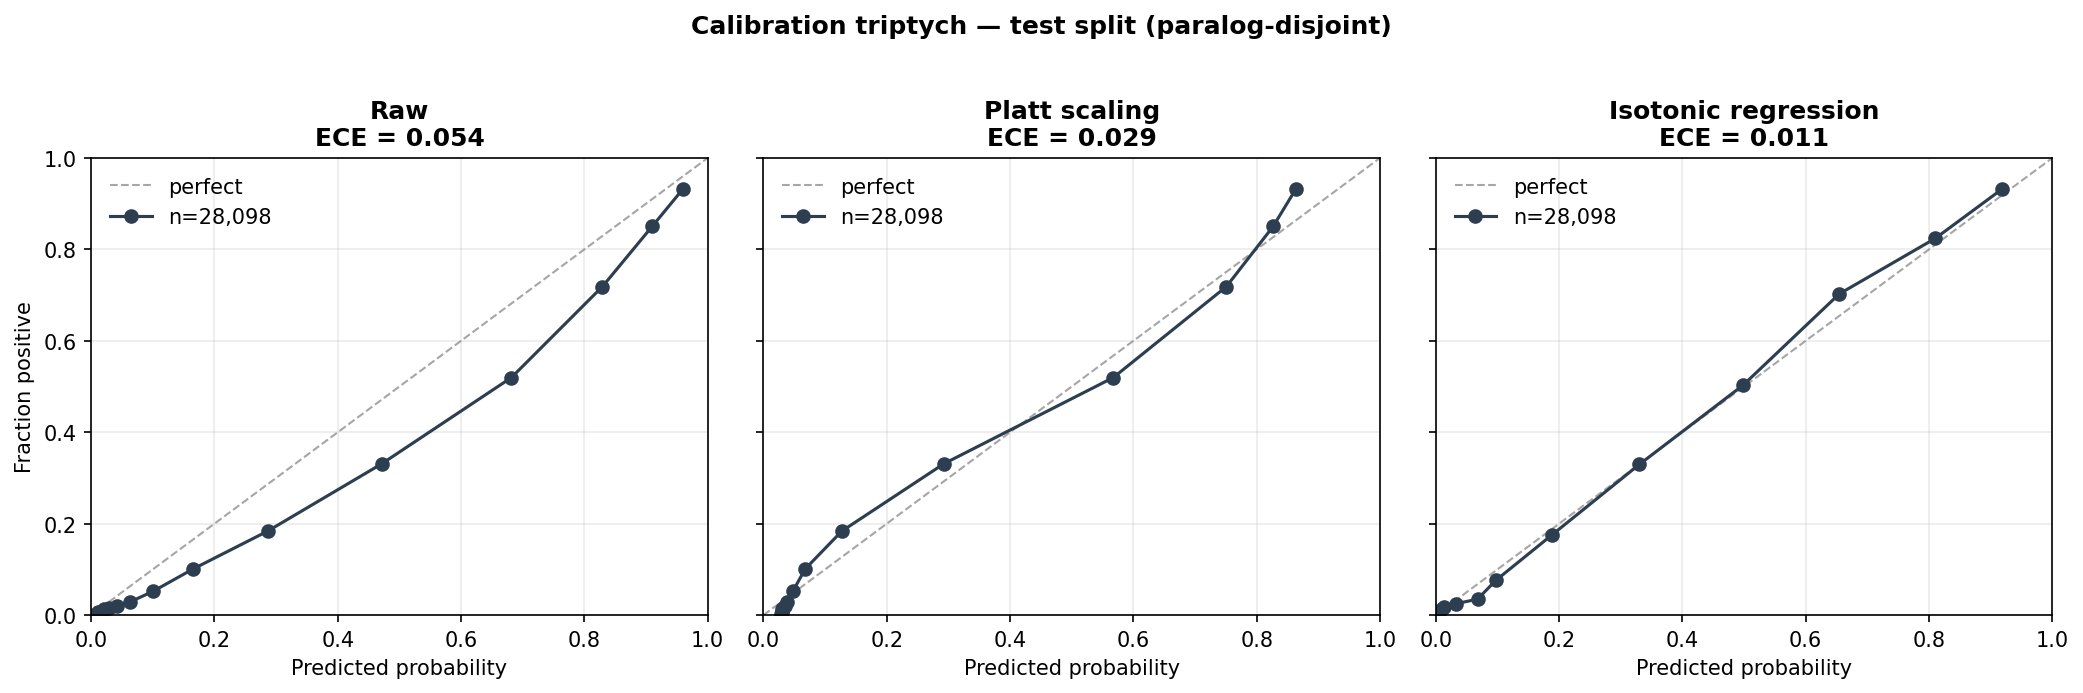
\includegraphics[width=\linewidth]{figures/calibration_triptych.png}
\end{frame}

% ═════════════════════════════════════════════════════════════════════════
% Part 5: Interpretability
% ═════════════════════════════════════════════════════════════════════════

\section{Interpretability}

\begin{frame}{SHAP --- what did the model actually learn?}
  TreeSHAP on a 2{,}000-variant stratified sample.
  \vspace{0.3em}
  \small
  \centering
  \begin{tabular}{@{} r l r @{}}
    \toprule
    Rank & Feature & mean $|$SHAP$|$ \\
    \midrule
    1 & phyloP100way\_vertebrate & 0.809 \\
    2 & AN (gnomAD allele number) & 0.532 \\
    \rowcolor{yellow!25}
    3 & \textbf{lof\_z} (gnomAD constraint) & 0.342 \\
    4 & alt\_aa\_P (Proline substitution) & 0.304 \\
    5 & pfam\_domain & 0.284 \\
    6 & phastCons100way\_vertebrate & 0.245 \\
    \rowcolor{yellow!25}
    8 & \textbf{oe\_mis\_upper} (gnomAD constraint) & 0.189 \\
    \bottomrule
  \end{tabular}
  \vspace{0.5em}
  \begin{itemize}
    \item \alert{Two Phase 2.1 additions (yellow) ranked \#3 and \#8}
          --- validating the hypothesis that gene-level priors are
          orthogonal signal.
  \end{itemize}
\end{frame}

\begin{frame}{SHAP beeswarm}
  \centering
  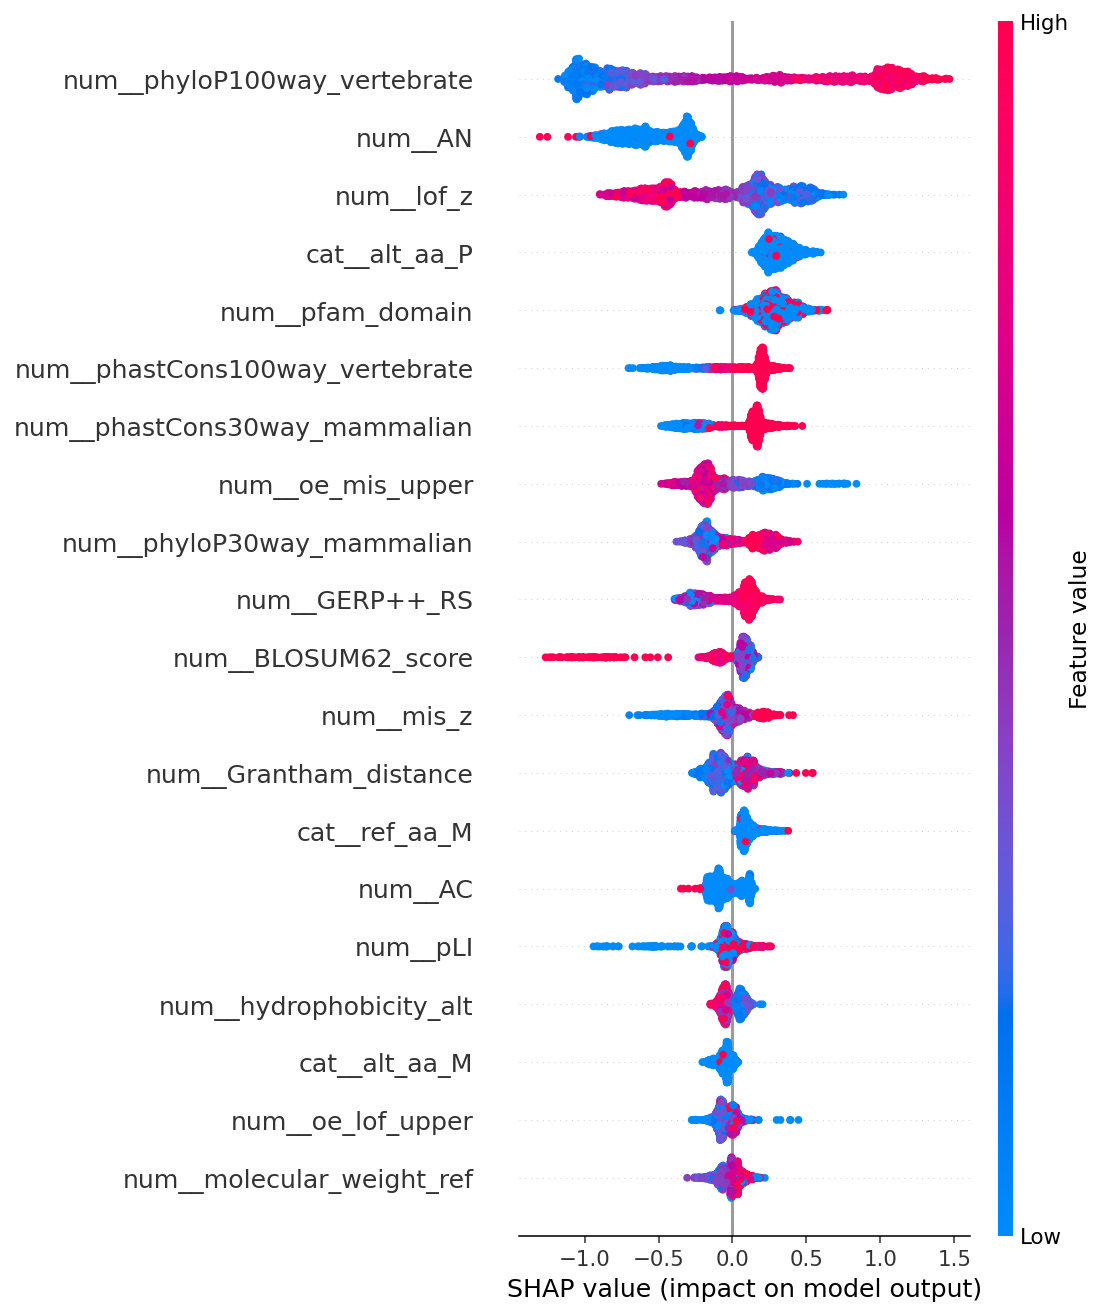
\includegraphics[width=0.7\linewidth]{figures/shap_summary.png}
\end{frame}

\begin{frame}{Confident errors}
  326 of 2{,}000 test variants (16.3\%) scored with
  $|p_{\text{cal}} - y| > 0.5$.
  \vspace{0.5em}
  \begin{itemize}
    \item \textcolor{alert}{264 false negatives} --- pathogenic
          variants scored confidently benign.
    \item \textcolor{subtle}{62 false positives} --- benign variants
          scored confidently pathogenic.
    \item FN-heavy pattern $\Rightarrow$ the remaining hard cases
          are low-conservation pathogenic variants.
    \item Every row of \texttt{confident\_errors.csv} carries its
          top-3 SHAP contributors for per-row attribution.
  \end{itemize}
\end{frame}

% ═════════════════════════════════════════════════════════════════════════
% Part 6: External validation
% ═════════════════════════════════════════════════════════════════════════

\section{External validation}

\begin{frame}{The real test: denovo-db}
  \begin{itemize}
    \item \textsc{denovo-db}: de-novo variants in affected children
          (autism, DD, epilepsy, CHD, schizophrenia) + sibling
          controls.
    \item Nearly every missense variant here ``looks damaging'' at
          the variant level.
    \item Separating causative from bystander requires
          \emph{gene-level} context.
  \end{itemize}
  \begin{alertblock}{The first result was sobering}
    \centering
    \large Before constraint features: \textbf{ROC-AUC 0.487}
    on unseen families. \\ \vspace{0.3em}
    \textbf{\emph{At chance.}}
  \end{alertblock}
\end{frame}

\begin{frame}{Before \vs after gnomAD gene-level constraint}
  \small
  \centering
  \begin{tabular}{@{} l r r l l @{}}
    \toprule
    Slice & $n$ & $n_+$ & ROC-AUC & PR-AUC \\
    \midrule
    full (pre)       & 642 & 498 & 0.468 [0.415, 0.519] & 0.761 \\
    full (post)      & 642 & 498 & \textbf{0.511} [0.455, 0.564] & \textbf{0.790} \\
    \rowcolor{yellow!25}
    holdout (pre)    & 201 & 161 & 0.487 [0.383, 0.583] & 0.789 \\
    \rowcolor{yellow!25}
    \textbf{holdout (post)} & 201 & 161 & \textbf{0.573} [0.476, 0.670] & \textbf{0.838} \\
    \bottomrule
  \end{tabular}
  \vspace{0.7em}
  \begin{itemize}
    \item Family-holdout slice: variants whose gene family never
          appeared in training.
    \item \textbf{Gene-level priors close half the generalisation
          gap.}
    \item ROC jumps \textbf{+0.086}; PR-AUC now above the base
          rate by 0.037.
  \end{itemize}
\end{frame}

% ═════════════════════════════════════════════════════════════════════════
% Part 7: Future work
% ═════════════════════════════════════════════════════════════════════════

\section{What's next}

\begin{frame}{Phase 2 roadmap}
  In decreasing expected impact-per-effort:
  \begin{enumerate}
    \item \textbf{ESM-2 full-training-set integration.}
          Zero-shot proof-of-concept shows +0.015 ROC from
          cheap rank-fusion on unseen families.
          Full compute currently running on Colab T4 ($\sim$8 h).
    \item \textbf{AlphaFold2 structural features.}
          pLDDT, SASA, DSSP, residue depth, 5\AA{} neighbour count.
    \item \textbf{ProteinGym external validation.}
          Deep-mutational-scanning fitness scores on a whitelist
          of genes absent from our training.
    \item \textbf{Hybrid stacking.}
          Meta-learner on (XGBoost, ESM-2 LLR, AlphaFold features).
  \end{enumerate}
\end{frame}

% ═════════════════════════════════════════════════════════════════════════
% Part 8: Reproducibility
% ═════════════════════════════════════════════════════════════════════════

\section{Reproducibility}

\begin{frame}{The whole project is one command away}
  \vspace{0.5em}
  \begin{block}{Clone $\to$ run}
  \small
  \begin{verbatim}
git clone <repo>
cd Genetic-Mutation-Detection-project
docker build -t missense .
docker run --rm missense make test
docker run --rm missense make reproduce-headline
  \end{verbatim}
  \end{block}
  \vspace{0.3em}
  \begin{itemize}
    \item 287 package versions pinned in \texttt{requirements-lock.txt}.
    \item 158 pytest tests $+$ 55\% coverage gate.
    \item GitHub Actions runs tests $+$ linters on every push.
    \item Leakage gate (4 checks) runs both as CLI and pytest.
    \item 10 narrative notebooks (\texttt{00\_overview} to
          \texttt{09\_esm2\_zero\_shot}) all pass
          \texttt{jupyter nbconvert --execute}.
  \end{itemize}
\end{frame}

% ═════════════════════════════════════════════════════════════════════════
% Final slide
% ═════════════════════════════════════════════════════════════════════════

\begin{frame}{Take-home messages}
  \begin{enumerate}
    \item \textbf{Honest numbers beat inflated ones.}
          Our 0.838 PR-AUC has no known contamination; the
          pre-audit 0.955 had three.
    \item \textbf{Like-for-like baselines change the conversation.}
          Against same-test-same-rules comparison we beat the
          classical tools cleanly, sit below AlphaMissense under
          stricter methodology.
    \item \textbf{External generalisation is the real benchmark.}
          At chance on denovo-db without gene priors, above chance
          after --- and this is the diagnostic that motivates Phase
          2.
  \end{enumerate}
  \vspace{1em}
  \centering
  \small
  Code, tests, notebooks, Docker, LaTeX report, Streamlit demo: \\
  \url{github.com/RayanAlDwlah/Genetic-Mutation-Detection-project}
\end{frame}

\begin{frame}[plain]{}
  \vspace{2cm}
  \centering
  {\Huge Thank you.}\\[2em]
  {\Large Questions?}
\end{frame}

\end{document}
